\chapter{Introduction}
\label{chap:intro}


\section{Introduction}

The classic issue about Vehicle Routing Problem (VRP) is a well known \textit{NP-hard} ~\cite{Lenstra1981} optimization problem of high importance in different logistics; it consists in delivery goods to a set of customers geographically dispersed, using a fleet of vehicles that begin its route in the central depot. The problem consists in assigning to each vehicle a route with the objective of minimizing the transportation cost.

The cost generated in the transport of goods, such as the size of the fleet of vehicles maintenance, combustible, and so on, are significant due to the fact that to the transport processes are involved at all stages of production processes, accounting for 10\% to 20\% of the final product cost~\cite{toth_vehicle_2001}.

One of the first investigation that studied the vehicle routing problem took place in the year 1959. In that work, Dantzing and Ramser~\cite{Dantzing1959} analyzed an oil dispatching problem with trucks; that problem arise as a generalization of the classic traveling salesman problem (TSP), where the salesman has to visit a set of customers for only one time and then come back to the origin point, building a Hamiltonian road on the graph consisting of customers (vertices) and the possible paths between clients (edges).

Different variations of the VRP have been proposed with the aim of approaching the problem real contexts; these problems include the addition of variables and constraints. The figure below shows a diagram with the most popular variants of VRP.

\begin{figure}[!htbp]
  \begin{center}
    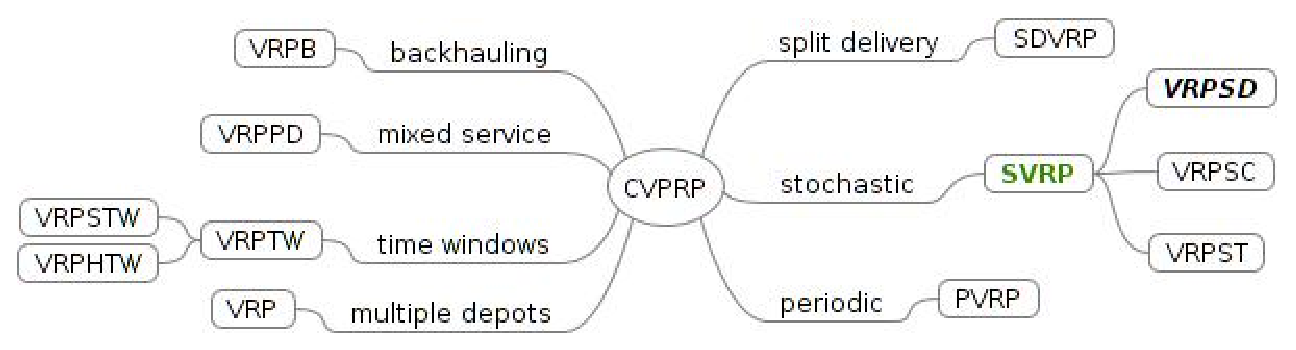
\includegraphics[width=0.8\textwidth]{Images/Chapter1/variants_vrp.eps}
  \end{center}
  \caption{Basic variants of the Vehicle Routing Problem}
  \label{fig:VRP_variants}
\end{figure}

When vehicle capacity is fixed, the Capacited Vehicle Routing Problem (CVRP) originates; if there are many depots, then we have Multiple Deposit Vehicle Routing Problem (MDVRP). The Split Delivery Vehicle Routing Problem (SDVRP) is a relaxation of the problem that allows a custumer to be served by several vehicles, being important in cases where the customer demand exceeds the vehicle capacity. Generally the VRP provide a planning for a fixed period and the Periodic Vehicle Routing Problem (PVRP) provides that planning for $m$ periods.

One of the most studied variants of the problem is caused by including time windows for deliveries, Vehicle Routing Problem with Time Windows (VRPTW), for this problem can be considered hard time windows (VRTHTW) were deliveries outside the established periods can not be done, and soft time windows (VRPSTW) in which deliveries can be made outside these periods, but with a penalty.

The problems that include pick-up and delivery can be divided in Vehicle Routing Problem with Backhauls (VRPB) and Vehicle Routing Problem with Pick-Up and Delivery (VRPPD) in the VRPB the group of custumers is divided in two subgroups, for the first group, all pick-up's are made of some product, then the vehicle returns to the depot and the deliveries are realized to the second group of custumers.  In the VRPPD, the pick-up's and deliveries to customers are made simultaneously.

The Stochastic Vehicle Routing Problem (SVRP) arise when there is uncertainty about some of the components of the VRP, i.e., one or more variables are random. Usually these problems include Vehicle Routing Problem with Stochastic Customers (VRPSC) where customers appears randomly, the Vehicle Routing Problem with Stochastic Times (VRPST) where travel times are random and Vehicle Routing Problem with Stochastic Demands (VRPSD), where the customers demands are known only with a probability distribution.

The SVRP's differ from the deterministic VRP in many important aspects. The solution concept is different, since many properties of the deterministic problem are not manageable in the stochastic case and solution methodologies are considerably more complex; hence, SVRP is often considered a computationally intractable problem and only small instances can be solved optimally and algorithms are difficult to design and evaluate~\cite{gendreau_stochastic_1996}.

The SVRP is either often modeled in the framework of stochastic programming (optimization) integer or mixed or as a Markov decision process. In stochastic programming, problems are usually modeled as two-stage, as chance constrained program (CCP) or as a stochastic program with recourse (SPR).

The VRPSD is an open problem of great importance in logistics owing to the diversity of real situations it represents. This problem occurs in the delivery of home heating oil~\cite{dror_computational_1985} in which each customer maintains a local inventory of the product and consumes an amount of oil each day; therefore, each day a fleet of trucks is dispatched to resupply a subset of customers. Stochastic demands are also evident in the collection of money by the vehicles of values, e.g. when collect money by a central bank ~\cite{jianhua_fan_multiple_2006} from several but not all of its branches every day; here the capacity of the vehicle used may be constrained for an upper bound on the amount of money that a vehicle might carry for safety reasons. The distribution of demand at each certain branch may be different, associated with the amount of money it handles. Other VRPSDs arise in delivering the post to large customers~\cite{Markovic_2005}, vending machines~\cite{yang_stochastic_2000} or delivering medical supplies in response to large-scale emergency~\cite{dessouky_rapid_2006}, or in recycling and waste management, among others.

\section{Proposal}

To design a hybrid evolutionary algorithm which combine stochastic dynamic optimization operators to find solutions for the vehicle routing problem with stochastic demands. Moreover, to evaluate the algorithm performance.


\section{Objective}

To design and test a hybrid evolutionary algorithm - Stochastic Dynamic Optimization (SDO) operator for the vehicle routing problem with stochastic demands.

\subsection{Specifics objectives}

\begin{enumerate}
 \item To analyze the alternatives for modeling and representing the problem, and select the most computationally convenient one.
 \item To design evolutionary and stochastic dynamic optimization operator algorithm to solve VRPSD.
 \item To implement the designed algorithm.
 \item To select benchmarking problems instances and alternative algorithms for testing.
 \item To develop experimental analyses and comparisons.
\end{enumerate}

\section{Contributions}

The evolutionary algorithms have not been broadly used to solve the vehicle routing problem with stochastic demands; thus, a hybrid evolutionary algorithm which combine stochastic dynamic optimization operators is proposed. This contribute with a new methodology to deal with the problem.

\subsection{Divulgation}


We presented this work at the Euro Conference in Stochastic Programming - ECSP 2014 which took place in Paris on Octuber, 2014. The  paper titled ``A hybrid local rollout dynamic programming global evolutionary algorithm for the vehicle routing problem with stochastic demands'' will be published in an special issue of the journal INFORMATICA with the contributions given at this conference.

\section{Outline}

In this first chapter a summary of the issues to be addressed was carried out, in chapter 2 presents the background and the state of the art of the VRPSD; chapter 3 presents the methodology used and the proposed algorithm. Chapter 4 presents the experiments and the numerical results and compares and discuss the results. Finally, chapter 5 presents the conclusions of the study.

